\chapter{Máquinas simples: alavancas, roldanas, planos inclinados}\label{ch:g5:simple-machines}

Sem motor, sem eletricidade --- e mesmo assim, com algumas vigas,
cordas e rampas, os construtores antigos levantaram pedras que juntas
de bois inteiras não conseguiam arrastar. A caixa de ferramentas
deles guardava as \emph{\omterm{def:g5:simple-machines:machine}{máquinas simples}}: invenções sem motor
nenhum, que transformam um puxão fraco e confortável num puxão
possante. Você já é dono da primeira; conheça a família.

\section{A família das poupadoras de esforço}

\begin{definition}[Máquina simples]\label{def:g5:simple-machines:machine}
Uma \emph{máquina simples}\index{máquina simples} é um dispositivo
sem motor que muda uma \omterm{def:g2:pushes-and-pulls:force}{força} para nos servir: tornando-a mais forte,
ou mudando a direção dela, ou as duas coisas. As clássicas: a
\emph{\omterm{def:g3:levers-and-scales:lever}{alavanca}}, que você conhece da gangorra e do pé de cabra, a
\emph{\omterm{def:g5:simple-machines:pulley}{roldana}} e o \emph{\omterm{def:g5:simple-machines:ramp}{plano inclinado}} --- a humilde rampa.
\end{definition}

\begin{example}[A alavanca, revisitada]\label{ex:g5:simple-machines:lever}
A regra da \omterm{def:g3:levers-and-scales:lever}{alavanca} você já tem: moedas vezes marcas --- a sua \omterm{def:g2:pushes-and-pulls:force}{força}
pequena longe do \omterm{def:g3:levers-and-scales:lever}{ponto de apoio} vence uma carga grande perto dele.
Repare agora em outra coisa: a sua ponta do pé de cabra desce um
caminho longo, enquanto o pedregulho sobe só um pouquinho. Guarde
essa observação no bolso; ela está prestes a virar uma lei.
\end{example}

\section{Roldanas}

\begin{definition}[Roldana]\label{def:g5:simple-machines:pulley}
Uma \emph{roldana}\index{roldana} é uma roda com um sulco para a
corda. Uma roldana \emph{fixa} fica pendurada numa viga e muda apenas
a direção do puxão: puxe para baixo e a carga sobe. Uma roldana
\emph{móvel} viaja na corda, com a carga pendurada nela: a carga fica
então pendurada em \emph{dois} trechos de corda, e cada trecho
carrega só metade do \omterm{def:g4:weight-and-mass:weight}{peso}.
\end{definition}

\begin{omfigure}
\begin{tikzpicture}[scale=0.8]
  \draw[thick] (0.2,4.4) -- (2.8,4.4);
  \draw[thick] (1.5,4.4) circle (0.42);
  \draw[thick] (1.08,4.4) -- (1.08,1.6);
  \draw[thick] (1.92,4.4) -- (1.92,2.8);
  \draw[thick, fill=omMeth, fill opacity=0.4]
    (0.68,0.8) rectangle (1.48,1.6);
  \node[font=\footnotesize] at (1.08,1.2) {carga};
  \draw[-Stealth, very thick, omThm] (1.92,2.8) -- (1.92,1.9);
  \node[right, font=\small] at (2.1,2.3) {puxão inteiro, para baixo};
  \node[below, font=\small] at (1.5,0.3) {fixa: muda a direção};
  \begin{scope}[xshift=6.6cm]
    \draw[thick] (0.2,4.4) -- (3.6,4.4);
    \draw[thick] (0.9,4.4) -- (0.9,2.2);
    \draw[thick] (1.74,2.2) circle (0.42) ;
    \draw[thick] (0.9,2.2) arc (180:360:0.42);
    \draw[thick] (2.58,2.2) -- (2.58,4.4);
    \draw[thick] (2.58,3.4) -- (2.58,4.4);
    \draw[thick] (1.74,1.78) -- (1.74,1.5);
    \draw[thick, fill=omMeth, fill opacity=0.4]
      (1.34,0.7) rectangle (2.14,1.5);
    \node[font=\footnotesize] at (1.74,1.1) {carga};
    \draw[-Stealth, very thick, omThm] (2.58,4.4) -- (2.58,4.9);
    \node[right, font=\small] at (2.75,4.6) {metade do puxão};
    \node[below, font=\small] at (1.9,0.3)
      {móvel: dois trechos dividem a carga};
  \end{scope}
\end{tikzpicture}

{\small Duas \omterm{def:g5:simple-machines:pulley}{roldanas}, dois presentes. A \omterm{def:g5:simple-machines:pulley}{roldana} fixa vira o seu
puxão de lado; a \omterm{def:g5:simple-machines:pulley}{roldana} móvel deixa dois trechos de corda dividirem
a carga, de modo que a sua mão segura só a metade.}
\end{omfigure}

\begin{omfigure}
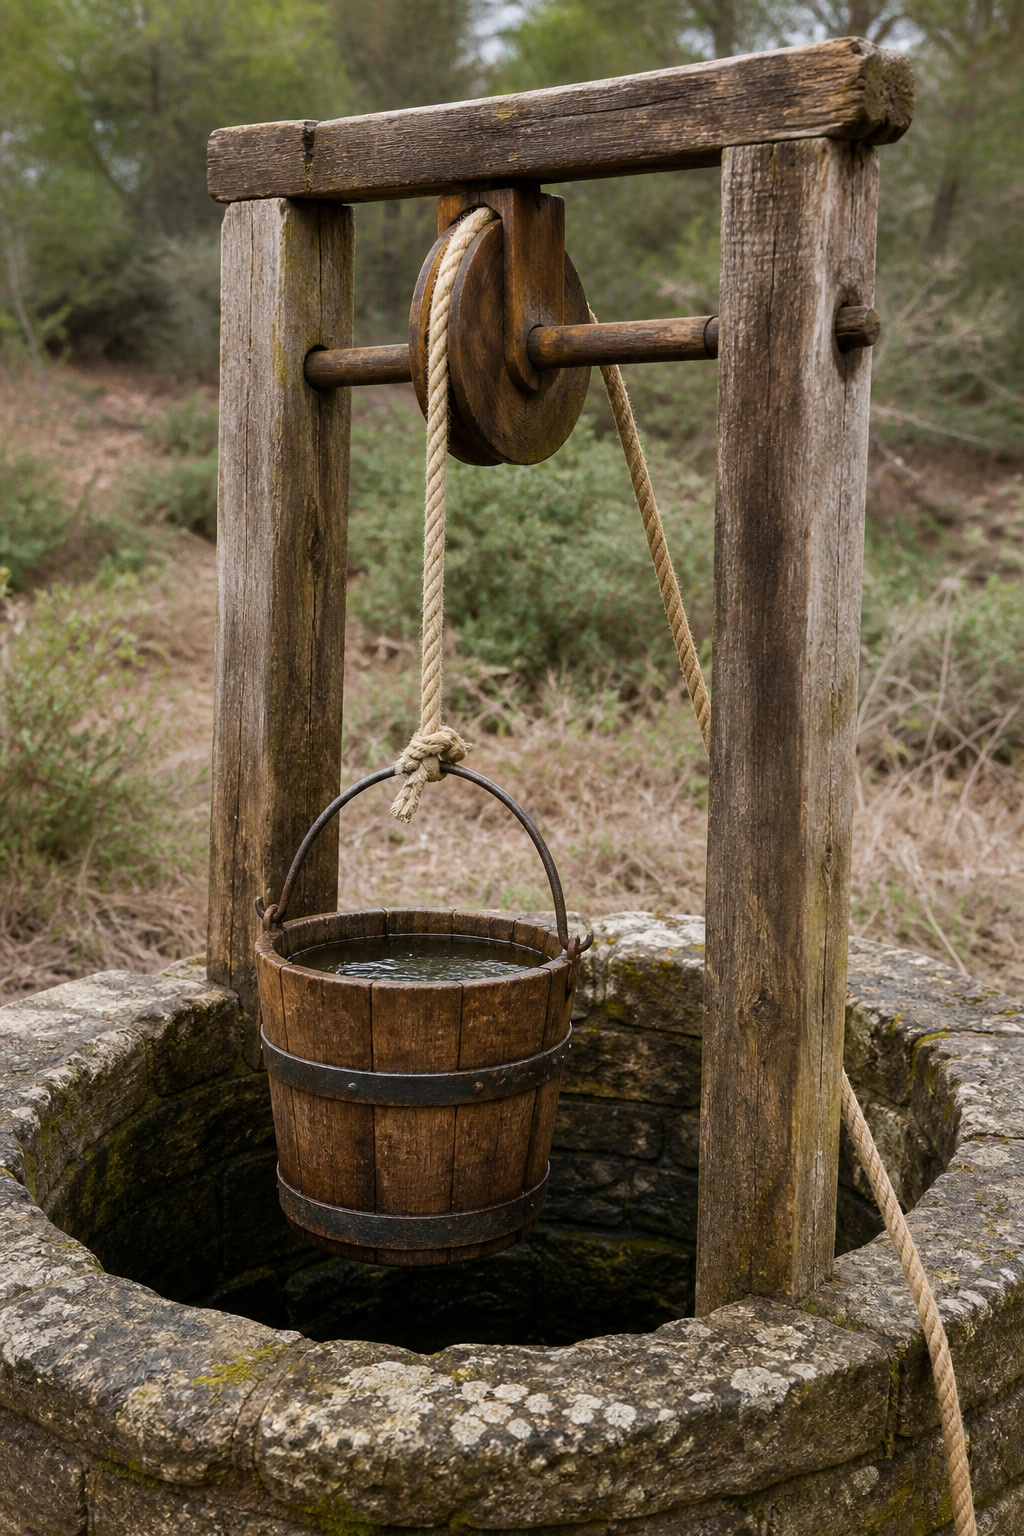
\includegraphics[width=0.34\linewidth]{images/book1/ai/g5-machines-pulley.jpg}

{\small A \omterm{def:g5:simple-machines:pulley}{roldana} do poço: a corda corre no sulco, e um puxão para baixo vira uma subida.}
\end{omfigure}

\begin{example}[Roldanas em ação]\label{ex:g5:simple-machines:pulleywork}
A bandeira sobe pelo mastro enquanto as suas mãos puxam
confortavelmente \emph{para baixo}: uma \omterm{def:g5:simple-machines:pulley}{roldana} fixa lá no alto ---
direção mudada, esforço igual, mas puxar para baixo deixa o seu
próprio \omterm{def:g4:weight-and-mass:weight}{peso} ajudar. A talha do construtor emenda várias \omterm{def:g5:simple-machines:pulley}{roldanas} de
modo que a carga fique pendurada em quatro ou seis trechos: cada
trecho carrega um quarto ou um sexto do \omterm{def:g4:weight-and-mass:weight}{peso}, e um único trabalhador
levanta um piano. Repare no trabalhador, porém: \omterm{def:g2:measuring-length:units}{metro} após \omterm{def:g2:measuring-length:units}{metro} de
corda corre pelas mãos dele, enquanto o piano sobe devagarinho.
\end{example}

\section{O plano inclinado}

\begin{definition}[Plano inclinado]\label{def:g5:simple-machines:ramp}
Um \emph{plano inclinado}\index{plano inclinado} --- uma rampa --- é
uma ladeira para levantar cargas sem erguê-las direto para cima.
Quanto mais suave a ladeira, menor o empurrão necessário para mover a
carga por ela: rolar um barril por uma rampa longa e suave é fácil;
por uma rampa curta e íngreme, brutal; direto para cima, impossível.
\end{definition}

\begin{method}[Sinta com a balança de elástico]\label{met:g5:simple-machines:measure}
A sua balança de elástico do ano passado consegue provar a diferença:
\begin{enumerate}
  \item ponha um carrinho de brinquedo numa tábua e prenda o elástico
        nele;
  \item apoie a tábua como uma rampa suave sobre uma \omterm{def:g3:first-electric-circuit:battery}{pilha} baixa de
        livros; arraste o carrinho devagar pelo elástico e anote o
        esticão;
  \item apoie a mesma tábua bem mais inclinada, sobre o assento de
        uma cadeira, e arraste de novo.
\end{enumerate}
O arrasto na rampa íngreme estica muito mais o elástico: ladeira mais
inclinada, esforço maior. As ladeiras suaves são mesmo suaves --- o
seu instrumento confirma.
\end{method}

\begin{omfigure}
\begin{tikzpicture}[scale=0.8]
  \draw[thick] (0,0) -- (11.2,0);
  \draw[very thick, omDef] (0.3,0) -- (6.5,2.0);
  \draw[thick, fill=omMeth, fill opacity=0.4]
    (2.8,0.82) rectangle ++(0.8,0.55);
  \draw[-Stealth, thick, omThm] (3.75,1.35) -- (4.65,1.64);
  \node[above, font=\small, omThm] at (3.4,1.75) {empurrão pequeno};
  \draw[very thick, omDef] (8.2,0) -- (10.2,2.0);
  \draw[thick, fill=omMeth, fill opacity=0.4]
    (8.75,0.5) rectangle ++(0.8,0.55);
  \draw[-Stealth, very thick, omThm] (9.75,1.25) -- (10.55,2.05);
  \node[above, font=\small, omThm] at (9.3,1.9) {empurrão grande};
  \node[below, font=\small] at (3.4,-0.3)
    {rampa longa e suave até a mesma altura};
  \node[below, font=\small] at (9.3,-0.3) {rampa curta e íngreme};
\end{tikzpicture}

{\small Mesmo caixote, mesma altura a ganhar: a rampa longa e suave
pede um empurrão pequeno num caminho longo; a rampa íngreme, um
empurrão grande num caminho curto.}
\end{omfigure}

\begin{example}[Rampas na paisagem]\label{ex:g5:simple-machines:ramps}
As rampas para cadeira de rodas correm longas e suaves ao lado de
escadas curtas --- suavidade de propósito. As estradas de montanha
ziguezagueiam: em vez de atacar o cume direto para cima, elas
enrolam um \omterm{def:g5:simple-machines:ramp}{plano inclinado} longo e suave para lá e para cá pela
encosta. E o parafuso é uma rampa disfarçada --- uma ladeira enrolada
em torno de uma haste, de modo que cada volta fácil da chave de fenda
enfia o parafuso um pouquinho mais fundo.
\end{example}

\section{A regra de ouro}

\begin{proposition}[A regra de ouro das máquinas]\label{prop:g5:simple-machines:golden}
Nenhuma \omterm{def:g5:simple-machines:machine}{máquina simples} dá alguma coisa de graça: tudo o que ela
poupa em \omterm{def:g2:pushes-and-pulls:force}{força}, ela cobra de volta em distância. Metade da \omterm{def:g2:pushes-and-pulls:force}{força} ---
o dobro de corda puxada, ou o dobro de caminho percorrido; um décimo
da \omterm{def:g2:pushes-and-pulls:force}{força} --- dez vezes o caminho. Máquina após máquina, a troca é
exata: o conforto é comprado com \omterm{def:g2:measuring-length:units}{metros}.
\end{proposition}

\begin{example}[Conferindo a regra]\label{ex:g5:simple-machines:check}
A \omterm{def:g5:simple-machines:pulley}{roldana} móvel: a sua mão puxa com metade da \omterm{def:g2:pushes-and-pulls:force}{força} e, para levantar
a carga \qty{1}{m}, você recolhe \qty{2}{m} de corda --- os dois
trechos precisam encurtar um \omterm{def:g2:measuring-length:units}{metro}. O pé de cabra: a sua ponta
percorre um arco comprido, o pedregulho mal se mexe. A rampa: o
caixote chega à mesma altura, mas você o empurrou pela ladeira
inteira. Toda economia paga, com precisão.
\end{example}

\begin{remark}[Por que a regra não pode ser burlada]\label{rem:g5:simple-machines:whygolden}
Escondida sob a regra de ouro está a nossa velha amiga do capítulo da
\omterm{def:g5:everyday-energy:energy}{energia}: levantar uma carga até uma altura custa uma porção fixa de
\omterm{def:g5:everyday-energy:energy}{energia}, e nenhum arranjo de cordas e tábuas muda o preço. As
máquinas só deixam você pagar em moedas menores --- em maior número.
Uma \omterm{def:g2:pushes-and-pulls:force}{força} pequena por um caminho longo entrega a mesma \omterm{def:g5:everyday-energy:energy}{energia} que
uma \omterm{def:g2:pushes-and-pulls:force}{força} grande por um caminho curto. As máquinas eternas
fracassaram exatamente por isso: a conta é sempre a conta.
\end{remark}

\section{Exercícios}

\begin{exercise}[$\star$]\label{exo:g5:simple-machines:1}
Diga as três \omterm{def:g5:simple-machines:machine}{máquinas simples} clássicas e um lugar do dia a dia em
que cada uma aparece.
\end{exercise}

\begin{exercise}[$\star$]\label{exo:g5:simple-machines:2}
O que uma \omterm{def:g5:simple-machines:pulley}{roldana} fixa muda no seu puxão? E o que uma \omterm{def:g5:simple-machines:pulley}{roldana} móvel
muda?
\end{exercise}

\begin{exercise}[$\star$]\label{exo:g5:simple-machines:3}
Por que puxar uma bandeira \emph{para baixo} para fazê-la subir é
mais confortável do que erguer o mesmo \omterm{def:g4:weight-and-mass:weight}{peso} direto para cima, mesmo
que o esforço tenha o mesmo tamanho?
\end{exercise}

\begin{exercise}[$\star$]\label{exo:g5:simple-machines:4}
Com uma \omterm{def:g5:simple-machines:pulley}{roldana} móvel, a carga fica pendurada em dois trechos. Que
parte do \omterm{def:g4:weight-and-mass:weight}{peso} a sua mão segura? Para levantar a carga \qty{3}{m},
quanta corda você precisa puxar?
\end{exercise}

\begin{exercise}[$\star$]\label{exo:g5:simple-machines:5}
No \cref{met:g5:simple-machines:measure}, qual rampa estica mais o
elástico? O que paga pelo esticão menor da rampa suave?
\end{exercise}

\begin{exercise}[$\star$]\label{exo:g5:simple-machines:6}
Por que as estradas de montanha ziguezagueiam em vez de subir direto
pela encosta? Qual \omterm{def:g5:simple-machines:machine}{máquina simples} é a estrada inteira?
\end{exercise}

\begin{exercise}[$\star$]\label{exo:g5:simple-machines:7}
Enuncie a regra de ouro das máquinas. Uma máquina deixa você puxar
com um décimo da \omterm{def:g2:pushes-and-pulls:force}{força} --- o que ela cobra de você?
\end{exercise}

\begin{exercise}[$\star$]\label{exo:g5:simple-machines:8}
Como um parafuso é um \omterm{def:g5:simple-machines:ramp}{plano inclinado} disfarçado? O que faz o papel
do caminho longo e suave?
\end{exercise}

\begin{exercise}[$\star\star$]\label{exo:g5:simple-machines:9}
Uma talha pendura um piano em quatro trechos. Que fração do \omterm{def:g4:weight-and-mass:weight}{peso} do
piano a mão do trabalhador puxa? Para levantar o piano \qty{2}{m},
quantos \omterm{def:g2:measuring-length:units}{metros} de corda passam pelas mãos dele?
\end{exercise}

\begin{exercise}[$\star\star$]\label{exo:g5:simple-machines:10}
Uma rampa de carga tem \qty{6}{m} de comprimento e sobe \qty{1}{m};
empurrar um caixote por ela exige um empurrão modesto. Os
carregadores impacientes montam uma rampa nova de apenas \qty{3}{m}
até a mesma plataforma. Usando a regra de ouro, compare o empurrão
novo com o antigo --- e explique por que ``metade do caminho'' não
foi vantagem nenhuma.
\end{exercise}

\begin{exercise}[$\star\star$]\label{exo:g5:simple-machines:11}
Um anúncio oferece um conjunto de \omterm{def:g5:simple-machines:pulley}{roldanas} ``tão esperto que você
puxa um \omterm{def:g2:measuring-length:units}{metro} de corda com metade da \omterm{def:g2:pushes-and-pulls:force}{força} --- e a carga sobe um
\omterm{def:g2:measuring-length:units}{metro} inteiro''. Ponha a promessa em julgamento diante da regra de
ouro e da conta de \omterm{def:g5:everyday-energy:energy}{energia} da
\cref{rem:g5:simple-machines:whygolden}: algum arranjo de rodas e
cordas conseguiria cumpri-la?
\end{exercise}
